\documentclass[11pt]{article}
\usepackage[margin=1in]{geometry}
\usepackage{amsmath}
\usepackage{amssymb}
\usepackage{booktabs}
\usepackage{enumitem}
\usepackage{tikz}
\usetikzlibrary{arrows.meta,positioning,fit,calc}
\usepackage[hidelinks]{hyperref}

\setlength{\parindent}{0pt}
\setlength{\parskip}{0.75\baselineskip}
\setlength{\emergencystretch}{2em}
\sloppy
\raggedbottom

\begin{document}

\title{NeoCore16x32: A Dual-Issue 7-Stage In-Order CPU Core for ECP5 FPGAs}
\author{Dulat Sarbassov\\Independent project}
\date{February 18, 2026}
\maketitle

\begin{abstract}
NeoCore16x32 is a synthesizable SystemVerilog CPU core with 16-bit general-purpose registers, 32-bit addressing, variable-length instructions, and a dual-issue in-order pipeline. The implemented pipeline is \texttt{IF1\,$\rightarrow$\,IF2\,$\rightarrow$\,IB\,$\rightarrow$\,ID\,$\rightarrow$\,EX\,$\rightarrow$\,MEM\,$\rightarrow$\,WB}, where IB is a clocked 6-entry instruction queue and part of the architectural stage count. The memory model is logically unified (von Neumann) and physically dual-ported through one 128-bit instruction-fetch port and one 32-bit data port into a single memory space. This document summarizes the ISA, microarchitecture, memory conventions, RTL organization, verification workflow, measured simulation behavior, and FPGA implementation results from the repository.
\end{abstract}

\section{Introduction}
NeoCore16x32 is developed as a full-stack CPU project: ISA definition, assembler/linker tooling, synthesizable RTL, and simulation/FPGA flows. This paper describes the implemented architecture directly and uses measured data from the project verification flow.

\section{Architectural Summary}
\subsection{Programmer-visible state}
NeoCore16x32 exposes:
\begin{itemize}[leftmargin=*]
  \item 16 general-purpose registers (R0--R15), each 16 bits,
  \item a 32-bit program counter,
  \item status flags Z (zero) and V (overflow).
\end{itemize}
R0 is not hardwired to zero. Software conventions may assign special roles (for example R14 as stack pointer), but hardware treats all GPRs as general-purpose.

\subsection{Data model and endianness}
The architecture is big-endian for both instructions and data. Native data sizes are byte (8), halfword (16), and word (32) with byte addressing over a 32-bit address space.

\subsection{Top-level pipeline view}
\begin{figure}[h]
  \centering
  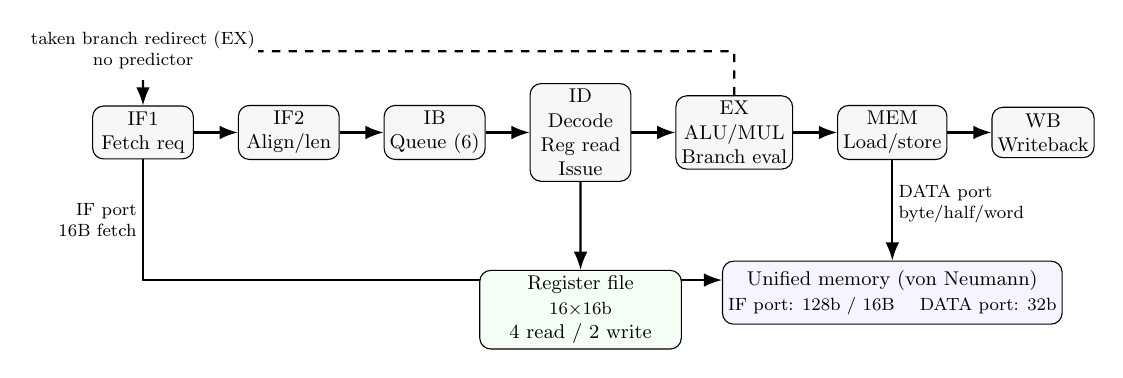
\begin{tikzpicture}[
    font=\small,
    box/.style={draw, rounded corners, align=center, minimum height=8mm, minimum width=16mm},
    stage/.style={box, fill=black!3},
    mem/.style={box, fill=blue!4, minimum width=42mm, minimum height=10mm},
    ann/.style={box, fill=green!4, minimum width=32mm, minimum height=10mm},
    arr/.style={-Latex, thick},
    darr/.style={-Latex, thick, dashed},
    every node/.style={inner sep=2.5pt},
    node distance=6mm and 7mm,
    scale=0.80,
    transform shape
  ]

    % --- Pipeline row (relative placement prevents overlap) ---
    \node[stage] (if1) {IF1\\Fetch req};
    \node[stage, right=of if1] (if2) {IF2\\Align/len};
    \node[stage, right=of if2] (ib)  {IB\\Queue (6)};
    \node[stage, right=of ib]  (id)  {ID\\Decode\\Reg read\\Issue};
    \node[stage, right=of id]  (ex)  {EX\\ALU/MUL\\Branch eval};
    \node[stage, right=of ex]  (memst) {MEM\\Load/store};
    \node[stage, right=of memst] (wb) {WB\\Writeback};

    \draw[arr] (if1.east) -- (if2.west);
    \draw[arr] (if2.east) -- (ib.west);
    \draw[arr] (ib.east)  -- (id.west);
    \draw[arr] (id.east)  -- (ex.west);
    \draw[arr] (ex.east)  -- (memst.west);
    \draw[arr] (memst.east) -- (wb.west);

    % --- Unified memory (below EX/MEM, centered, no overlap) ---
    \node[mem, below=16mm of memst] (umem)
      {Unified memory (von Neumann)\\\footnotesize IF port: 128b / 16B \quad DATA port: 32b};

    \draw[arr] (if1.south) |- node[pos=0.25, left, align=right, font=\footnotesize]{IF port\\16B fetch} ([yshift=2mm]umem.west);
    \draw[-, thick] (memst.south) |- node[pos=0.25, right, align=left, font=\footnotesize]{DATA port\\byte/half/word} ([yshift=2mm]umem.north -| memst.south) coordinate (mem2umem_end);
    \draw[arr] (mem2umem_end) -- (umem.north);

    % --- Register file (below ID) ---
    \node[ann, below=14mm of id] (rf)
      {Register file\\\footnotesize 16$\times$16b\\4 read / 2 write};
    \draw[arr] (id.south) -- (rf.north);

    % --- Branch redirect (resolved in EX; route above row cleanly) ---
    \coordinate (redirTop) at ($(ex.north)+(0,7mm)$);
    \draw[darr] (ex.north) -- (redirTop) -|
      node[pos=0.70, above, align=center, font=\footnotesize, fill=white, inner sep=1.5pt]{taken branch redirect (EX)\\no predictor} (if1.north);
  \end{tikzpicture}
  \caption{NeoCore16x32 block diagram. The 7-stage in-order pipeline is dual-issue; branches are resolved in EX (no predictor).}
\end{figure}

\section{Instruction Set and Encoding}
\subsection{ISA scope}
The ISA defines 26 opcodes, organized across ALU, MOV, branch/control flow, multiply, stack, subroutine, and control classes. Instruction length is variable from 2 to 9 bytes.

\subsection{Common instruction prefix}
All instructions begin with:
\begin{itemize}[leftmargin=*]
  \item Byte 0: \textbf{specifier} (mode/variant and length behavior),
  \item Byte 1: \textbf{opcode}.
\end{itemize}
Remaining bytes encode register fields and big-endian immediates/addresses.

\subsection{Concrete encoding example}
A representative register-format ALU instruction is:
\begin{center}
\begin{tabular}{@{}llll@{}}
\toprule
Byte 0 & Byte 1 & Byte 2 & Byte 3 \\
\midrule
Specifier & Opcode & \texttt{rd} & \texttt{rn} \\
\bottomrule
\end{tabular}
\end{center}

Register IDs are carried in the low nibble of Byte 2 (\texttt{rd}) and Byte 3 (\texttt{rn}).

Example (\texttt{ADD} register mode): \texttt{ADD R1, R2} is encoded as bytes
\texttt{[0x01][0x01][0x01][0x02]}, where:
\begin{itemize}[leftmargin=*]
  \item Byte 0 \texttt{0x01}: register-mode specifier,
  \item Byte 1 \texttt{0x01}: \texttt{ADD} opcode,
  \item Byte 2 \texttt{0x01}: \texttt{rd = R1},
  \item Byte 3 \texttt{0x02}: \texttt{rn = R2}.
\end{itemize}
For this mode, the implemented arithmetic ordering is \texttt{rd := rn + rd}, so the example executes as \texttt{R1 := R2 + R1}.

\section{Pipeline and Issue Microarchitecture}
\subsection{7-stage pipeline}
NeoCore16x32 uses:
\begin{center}
\texttt{IF1 $\rightarrow$ IF2 $\rightarrow$ IB $\rightarrow$ ID $\rightarrow$ EX $\rightarrow$ MEM $\rightarrow$ WB}
\end{center}

\begin{center}
\begin{tabular}{@{}ll@{}}
\toprule
Stage & Purpose \\
\midrule
IF1 & Fetch request / PC steering \\
IF2 & Fetch output / length predecode \\
IB & 6-entry instruction queue \\
ID & Decode, register read, issue decision \\
EX & ALU/multiply/branch execution \\
MEM & Load/store path \\
WB & Architectural writeback \\
\bottomrule
\end{tabular}
\end{center}

\subsection{Frontend design}
The fetch unit maintains a 64-byte sliding window using four 16-byte buffers (\texttt{buf\_hi}, \texttt{buf\_lo}, \texttt{buf\_pf}, \texttt{buf\_p2}) to support variable-length extraction and reduce boundary bubbles.

\subsection{Dual-issue rules (current RTL)}
Two instructions may issue together when all restrictions pass:
\begin{itemize}[leftmargin=*]
  \item no data-port structural conflict,
  \item no write-port conflict,
  \item no inter-pair data dependency that must serialize,
  \item no dual-branch pair (branch+non-branch is allowed),
  \item no UMULL/SMULL pairing restriction,
  \item no halt restriction.
\end{itemize}

Important current behavior: branch pairing is blocked only when \emph{both} instructions are branches. If slot 0 is a taken branch and slot 1 was issued, execute-stage logic squashes slot 1 side effects.

\subsection{Hazards and forwarding}
Hazard handling combines:
\begin{itemize}[leftmargin=*]
  \item register-file same-cycle forwarding,
  \item EX operand forwarding with priority EX/MEM $>$ MEM/WB $>$ WB,
  \item automatic stalls when forwarding cannot satisfy correctness.
\end{itemize}
A load-use dependency incurs a one-cycle stall in the current timing model. Load data is produced at the end of MEM and can be forwarded to EX in the following cycle.

\subsection{Control flow}
There is no branch predictor. Branches resolve in EX and taken branches flush frontend/decode state and redirect the fetch PC. The nominal taken-branch recovery is 3 cycles in the current configuration: after EX resolves the branch, IF1/IF2/IB are flushed and refilled, and the first valid target-path instruction reaches the frontend/decode boundary three cycles later.

\section{Unified Memory System}
The core uses a unified address space with two physical ports to one memory array:
\begin{itemize}[leftmargin=*]
  \item IF port: 128-bit (16-byte) fetch,
  \item DATA port: 32-bit load/store path with byte/halfword/word operations.
\end{itemize}
Default testbench memory size is 64 KiB. Access semantics are big-endian for all supported widths.

\section{Implementation Organization}
The implementation is partitioned into stage-local modules:
\begin{itemize}[leftmargin=*]
  \item frontend (fetch and instruction buffering),
  \item decode/issue (instruction decode, dependency checks, pairing),
  \item execution (ALU, multiply, branch evaluation),
  \item backend (memory access, writeback, register file),
  \item explicit pipeline-register boundaries between stages.
\end{itemize}

\section{Toolchain and Verification}
\subsection{Assembler/linker context}
The documentation references companion tools \texttt{nc16x32-as} and \texttt{nc16x32-ld} and a custom relocatable object format (LF02). The assembler flow is described as preprocess, lex, parse/semantic passes, encode, and serialize; linker flow performs section placement and relocation.

\subsection{RTL verification flow}
Primary verification steps are:
\begin{itemize}[leftmargin=*]
  \item \texttt{make unit-tests}
  \item \texttt{make core-tests}
  \item \texttt{make run\_any PROGRAM=mem/<file>.hex}
\end{itemize}

For profiling, the integration testbench exposes per-cycle counters with \texttt{+PROFILE}.

\section{Measured Simulation Performance}
To keep this section fully repository-grounded, results below were collected from \texttt{make run\_any ... VVPARGS=+PROFILE} in \texttt{tb/core\_any\_tb.sv}.

\begin{center}
\begin{tabular}{@{}lrrrr@{}}
\toprule
Workload & Cycles & Issued IPC & Dual-issue cycles & Taken branches / 100 issued inst. \\
\midrule
\texttt{mem/splitmix.hex} & 25 & 1.600 & 76.0\% & 0.0 \\
\texttt{mem/rle.hex} & 1276 & 1.047 & 43.2\% & 7.3 \\
\texttt{mem/test\_mixed\_lengths.hex} & 174587 & 0.729 & 18.5\% & 13.6 \\
\bottomrule
\end{tabular}
\end{center}

Additional profile highlights from \texttt{mem/test\_mixed\_lengths.hex}:
\begin{itemize}[leftmargin=*]
  \item Fetch IPC (valid): 1.063, IB IPC (valid): 0.987
  \item Issue rejects (both valid, no dual): 45153 (25.9\% of cycles)
  \item Main reject contributors: branch restrict 32.6\% of rejects, data dependency 29.2\%, write conflict 28.9\%
  \item Stall cycles: mem 6.1\%, hazard 0.0\% (rounded)
\end{itemize}

Restriction counters are not mutually exclusive; more than one reject condition can be true in the same cycle.

Theoretical peak throughput is 2.0 IPC; the measured workloads above span roughly 36\% to 80\% of that peak.

Repository \texttt{README.md} also reports directional Dhrystone-like performance around 23 MIPS at 25 MHz for a compact kernel setup.

\subsection{Dhrystone-style kernel report}
The project also tracks a Dhrystone-like run (1000 iterations) with the following measured counters:
\begin{center}
\begin{tabular}{@{}l r@{}}
\toprule
Metric & Value \\
\midrule
Program halt PC & \texttt{0x000000f7} \\
Total cycles & 68009 \\
IPC (issued) & 0.912 \\
Dual-issue cycles & 19009 (28.0\%) \\
Fetch IPC (valid) & 1.338 \\
IB IPC (valid) & 1.235 \\
Branch taken cycles & 6000 (8.8\%) \\
Issue rejects (both valid, no dual) & 22000 (32.3\%) \\
Stall cycles & mem=7001 (10.3\%), hazard=1000 (1.5\%) \\
\bottomrule
\end{tabular}
\end{center}

\textbf{Frontend behavior}
\begin{itemize}[leftmargin=*]
  \item Fetch dual-valid cycles: 43011 (63.2\%); IB dual-valid cycles: 41009 (60.3\%)
  \item Fetch bubbles (\texttt{valid0=0}): 20000 (29.4\%)
  \item IB blocked (\texttt{valid0 \& accept=0}): 12002 (17.6\%)
  \item Fetch \texttt{mem\_req} cycles: 39004 (57.4\%); fetch \texttt{mem\_ack} cycles: 39003 (57.3\%)
  \item Fetch no-HI-valid cycles: 10001 (14.7\%); fetch inst0-fits stalls: 3999 (5.9\%)
\end{itemize}

\textbf{Issue reject breakdown}
\begin{itemize}[leftmargin=*]
  \item mem conflict: 999 (1.5\% of cycles, 4.5\% of rejects)
  \item data dependency: 13000 (19.1\% of cycles, 59.1\% of rejects)
  \item write conflict: 8000 (11.8\% of cycles, 36.4\% of rejects)
  \item branch restrict: 4000 (5.9\% of cycles, 18.2\% of rejects)
  \item mul restrict: 0 (0.0\% of cycles, 0.0\% of rejects)
  \item halt restrict: 2001 (2.9\% of cycles, 9.1\% of rejects)
\end{itemize}

\section{FPGA Implementation Results (ECP5)}
Synthesis/place-and-route artifacts in this repository target ULX3S-85F (ECP5-85K, CABGA381) via Yosys/nextpnr.

From \texttt{build/nextpnr\_report.json}:
\begin{itemize}[leftmargin=*]
  \item Achieved $f_{\\mathrm{max}}$: 25.0388 MHz (constraint 25 MHz, pass)
  \item \texttt{DP16KD}: 64 / 208 (30\%)
  \item \texttt{MULT18X18D}: 3 / 156 (1\%)
  \item \texttt{TRELLIS\_COMB}: 12449 / 83640 (14\%)
  \item \texttt{TRELLIS\_FF}: 2225 / 83640 (2\%)
  \item \texttt{TRELLIS\_IO}: 17 / 365 (4\%)
\end{itemize}

The utilization profile is BRAM-heavy relative to LUT/FF, consistent with the wide fetch path and unified memory structure.

\section{Conclusion}
NeoCore16x32 demonstrates a practical dual-issue in-order core with variable-length encoding, deterministic 7-stage execution, and an FPGA-friendly implementation strategy. The design achieves useful IPC improvements from dual issue while keeping control and hazard behavior explicit and testable. The repository includes enough architecture, RTL, and profiling infrastructure to treat this core as a complete reference implementation for its ISA generation.

\section*{Reproducibility Commands}
\begin{itemize}[leftmargin=*]
  \item \texttt{make unit-tests}
  \item \texttt{make run\_any PROGRAM=mem/splitmix.hex VVPARGS=+PROFILE}
  \item \texttt{make run\_any PROGRAM=mem/rle.hex VVPARGS=+PROFILE}
  \item \texttt{make run\_any PROGRAM=mem/test\_mixed\_lengths.hex VVPARGS=+PROFILE}
  \item \texttt{make fpga} (for \texttt{build/nextpnr\_report.json})
\end{itemize}

\end{document}
